\chapter{Results}
\label{chap:results}
\begin{figure}[h!]
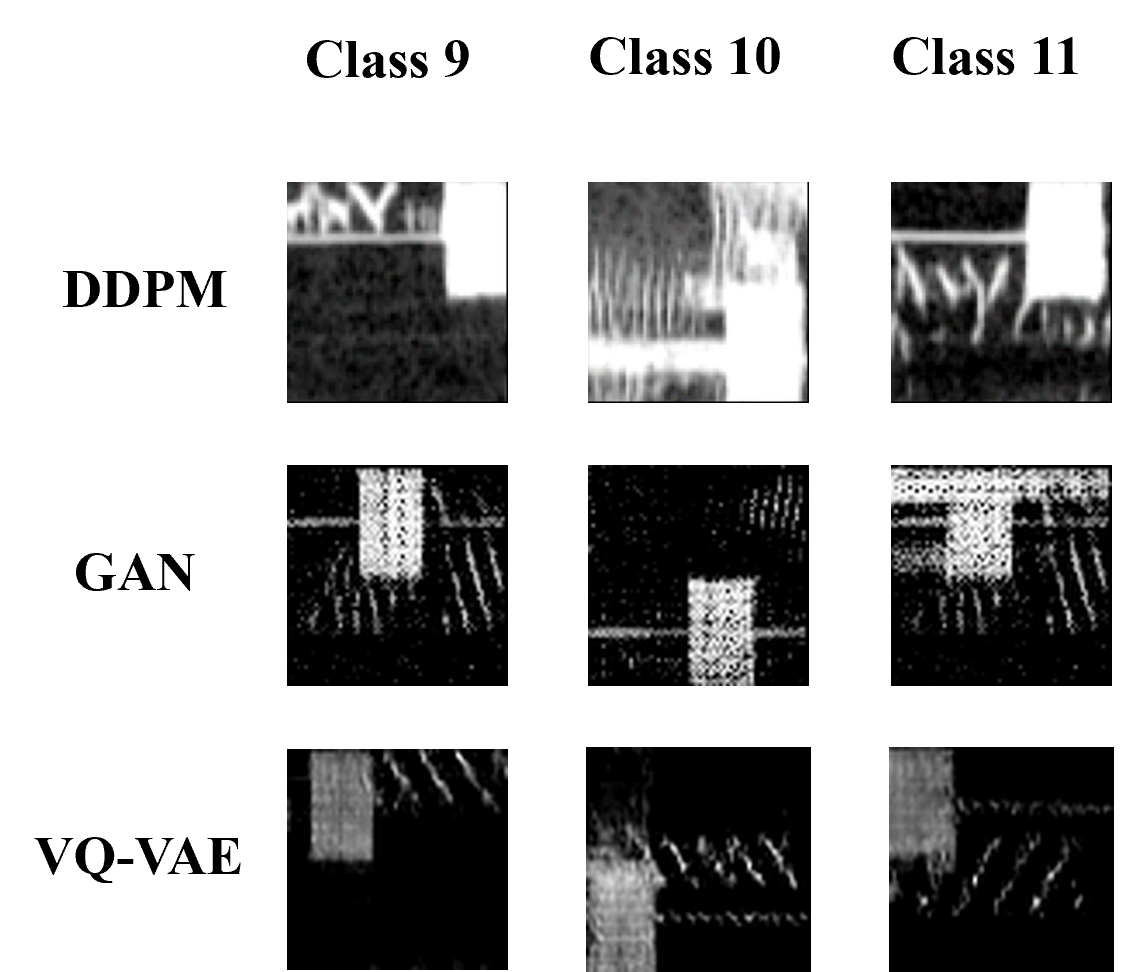
\includegraphics[width=10cm]{figures/Picture7.png}
\centering
\caption{A side-by-side comparison of some of the collision scenarios generated by the \gls{ddpm}, the \gls{gan}, and the \gls{vq-vae} }
\centering
\end{figure}

Classes depicted in Figure 3.1: class 9, class 10, and class 11 are all collision scenarios (Refer to Figure 2.1), which were generated by the 
\gls{ddpm}, the \gls{gan}, and the \gls{vq-vae}. 

\begin{figure*}[ht]
    \centering
    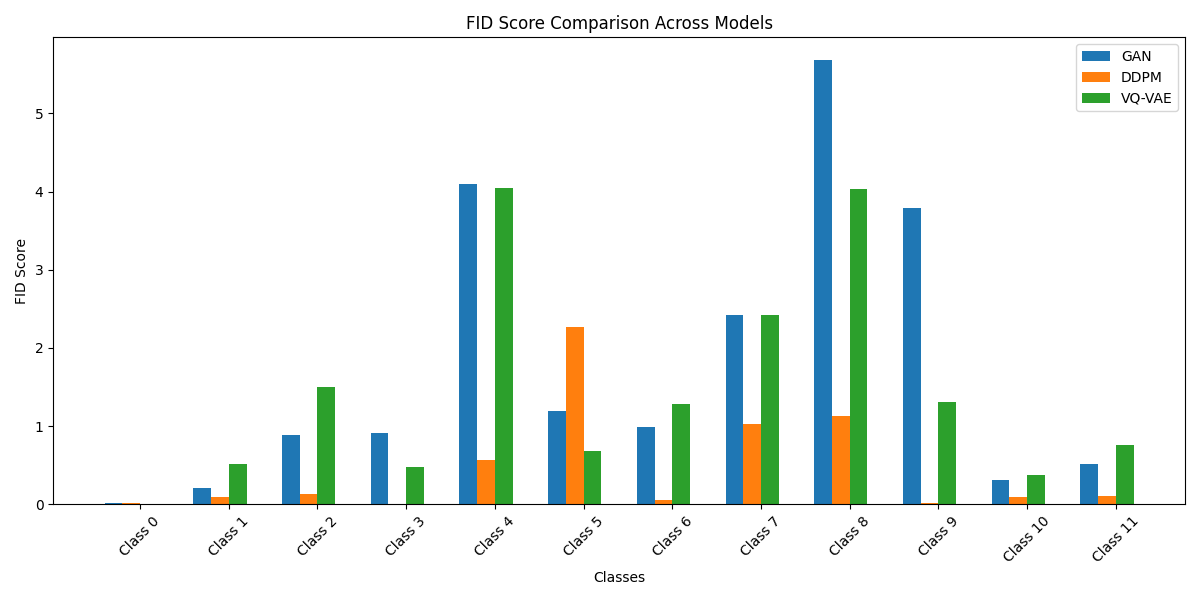
\includegraphics[width=\textwidth]{figures/Figure_12.png} 
    \caption{\gls{fid} Score Comparison Across Models for Different Classes.}
    \label{fig:fid_scores}
\end{figure*}
Figure 3.2 illustrates the change in \gls{fid} score across the classes for the 3 models.  The \gls{gan}, \gls{ddpm}, and \gls{vq-vae} models achieved 
average \gls{fid} scores of 1.944, 0.504, and 1.580, respectively. We used a ResNet18 model with the final classification layer replaced to extract 
features instead of using a pre-trained InceptionV3 network due to the specific nature of our dataset.

Since our dataset lacks the complex textures, patterns, and color information typically found in natural image datasets, the differences between real 
and generated spectrograms are smaller in the feature space. As a result, the \gls{fid} scores we obtained are smaller than usual for all three models.

Class 0 consistently shows near-zero \gls{fid} scores across all three models due to its purely noise-like nature. As observed in the graph, the classes 
representing collision scenarios—Class 9, Class 10, and Class 11—exhibit significantly lower \gls{fid} scores for images generated by the \gls{ddpm}. 
This suggests that the spectrogram images with collision scenarios generated by the \gls{ddpm} are more natural and resemble the original dataset better 
than the other two models. The other two models also have relatively low \gls{fid} scores for Class 10 and Class 11.

Among the three models, the \gls{ddpm} also has the lowest average \gls{fid} score, suggesting that \gls{ddpm} is the most effective model overall 
for generating spectrograms that closely resemble the real dataset, as evidenced by its consistently low \gls{fid} scores across most classes.

The \gls{gan} model's high \gls{fid} scores across many classes suggest model collapse in its generated spectrograms for this dataset, to which 
\gls{gan}s are susceptible. Given that our main focus is on generating a diverse dataset to improve the accuracy of a visualized interference 
classification system, having a wide variety of data is essential.

\gls{vq-vae} model, on the other hand, shows varied performance, outperforming \gls{gan} in many cases (e.g., Classes 1, 2, 6, 9) but 
falling behind \gls{ddpm} in most.

\begin{figure}[h]
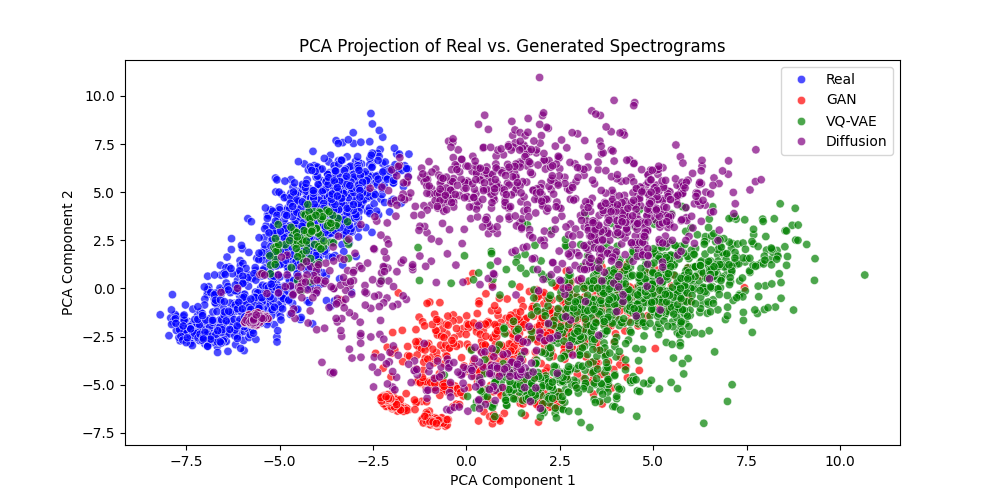
\includegraphics[width=\textwidth]{figures/PCA (1).png}
\centering
\caption{ \gls{pca} scores for the \gls{gan}, \gls{ddpm} and \gls{vq-vae}}
\centering
\end{figure}
The \gls{pca} projection in Figure 3.3 indicate that real and generated spectrograms form separate yet overlapping clusters, suggesting that generative models 
do not simply reproduce existing samples but introduce new variations. The spread of generated samples in the \gls{pca} projection indicates that the models 
create additional variations, potentially improving classifier generalization. The \gls{pca} analysis provides an independent validation of data distribution 
differences, confirming that generative models add meaningful diversity.
However, the \gls{pca} projection also shows that the \gls{gan} model's generated samples are more clustered and less spread out than the other two models, 
indicating that the \gls{gan} model may not be as effective at generating diverse samples as the \gls{ddpm} and \gls{vq-vae} models. The \gls{ddpm} model's 
generated samples are more spread out than the \gls{vq-vae} model's, suggesting that the \gls{ddpm} model may be more effective at generating diverse samples 
than the \gls{vq-vae} model.


\begin{figure}[t]
    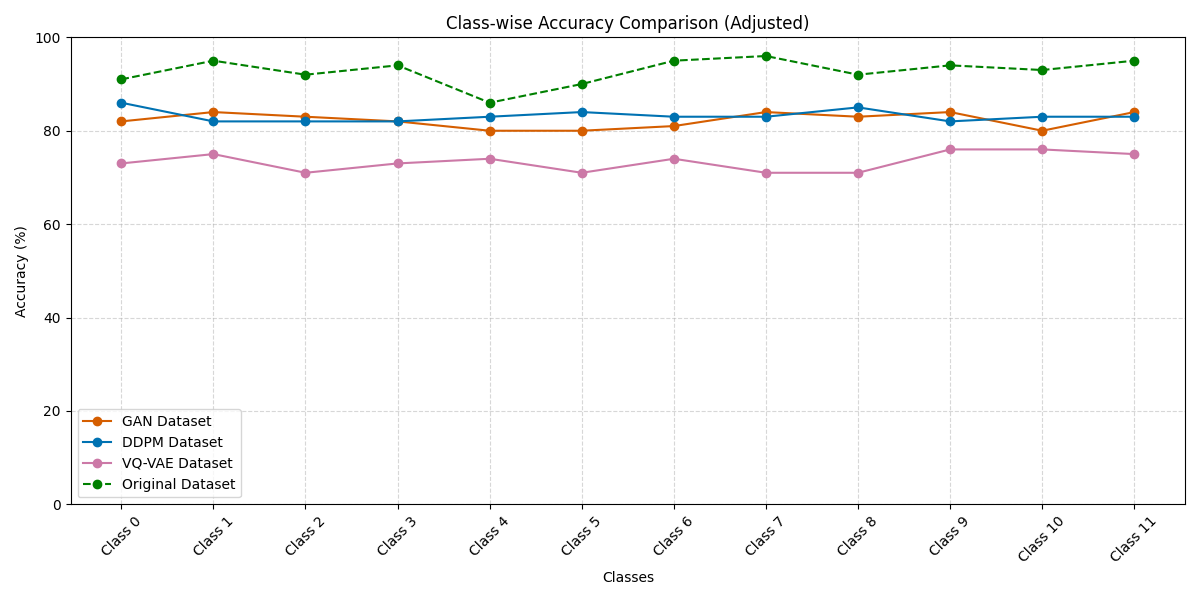
\includegraphics[width=8.5cm]{figures/final_graph.png}
    \centering
    \caption{Class-wise classification accuracy for \gls{gan}, \gls{ddpm}, \gls{vq-vae} generated data with original dataset}
    \centering
    \end{figure}
    
    Figure 3.4 illustrates the change in the classification accuracy of the \gls{cnn} model for the spectrogram images generated by the three generative 
    models for the twelve different data classes. Meanwhile, the spectrogram images generated by the \gls{ddpm} generally outperformed the images generated
    by other models. Even though we used a \gls{cnn} model specifically trained to distinguish fine-grained features ignoring the noise, the high noise and 
    blurry features in the \gls{vq-vae} model seem to have affected the accuracy of the \gls{cnn} model than the other two models. 
    
    
    \begin{table}[h!]
        \centering
        \begin{tabular}{c c c c}
            \hline
            Cases & Model & Average Accuracy & \gls{fid} Score \\
            \hline
            1 & \gls{ddpm} & 83.17\% & 0.504\\
            \hline
            2 & \gls{gan} & 82.75\% & 1.944\\
            \hline
            3 & \gls{vq-vae} & 73.25\%  & 1.580\\
            \hline
            4 & Original dataset & 92.75\%  & - \\
            \hline
        \end{tabular}
        \caption{Average accuracy for \gls{gan}, \gls{ddpm}, \gls{vq-vae} and Original data}
        \label{tab:average_accuracy}
    \end{table}
    
    Table 1 depicts the average classification accuracy and the \gls{fid} scores of the spectrogram images, for the three different models and the original data.
    Although the average accuracy is not far apart for the three generative models, due to the lack of diversity of the generated data by the \gls{gan}, and the noisy
     images by \gls{vq-vae} we can conclude that the \gls{ddpm} performs better than the \gls{gan} or \gls{vq-vae} when generating spectrogram images for a robust 
     spectrum-sharing system.
    
    We can also notice that the classification accuracy for the original dataset is much higher than the other three models. This is expected since the original dataset 
    is a real dataset. However, the \gls{ddpm} model's generated data is not far behind the original dataset, indicating that 
    the \gls{ddpm} model can generate high-quality spectrogram images that can be used to train a robust spectrum-sharing system. But when these models were
    directed to detect collisions in the simulated \gls{cbrs} environment all three generative models performed better than the original dataset. This is because 
    the original dataset was not diverse enough to train a robust \gls{cnn} model using data from a different domain.
    We will discuss this later in the chapter.
    
    After calculating the classification accuracy we trained four \gls{dqn} agents using the generated data from the three models and the original data. 
    The \gls{dqn} agents were trained for 1000 episodes. We then evaluated the trained \gls{dqn}agent based on how well the agent was able to avoid 
    collisions using the CNN classifications of the four models in the simulated MATLAB \gls{cbrs} environment.

    
\begin{figure}[htbp]
    \centering
    \begin{subfigure}[b]{0.45\textwidth}
        \centering
        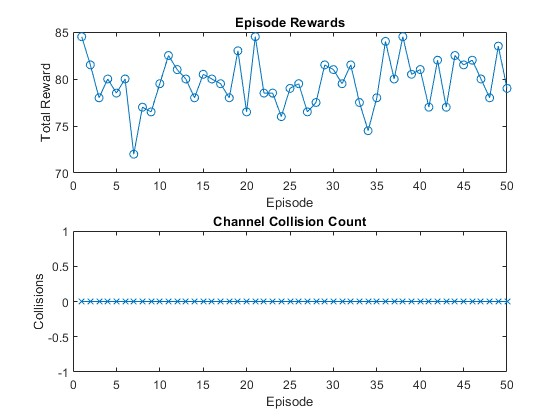
\includegraphics[width=\linewidth]{figures/collision_count_ddpm.jpg}
        \caption{DDPM}
    \end{subfigure}
    \hfill
    \begin{subfigure}[b]{0.45\textwidth}
        \centering
        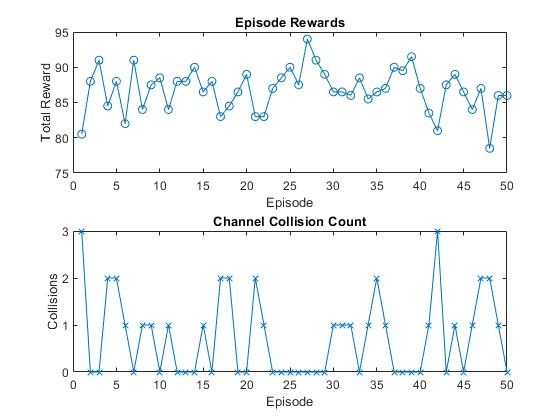
\includegraphics[width=\linewidth]{figures/collision_count_gan.jpg}
        \caption{GAN}
    \end{subfigure}

    \vspace{0.5cm} % space between rows

    \begin{subfigure}[b]{0.45\textwidth}
        \centering
        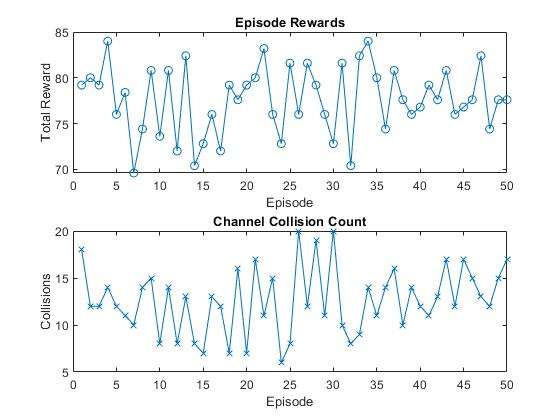
\includegraphics[width=\linewidth]{figures/collision_count_vqvae.jpg}
        \caption{VQ-VAE}
    \end{subfigure}
    \hfill
    \begin{subfigure}[b]{0.45\textwidth}
        \centering
        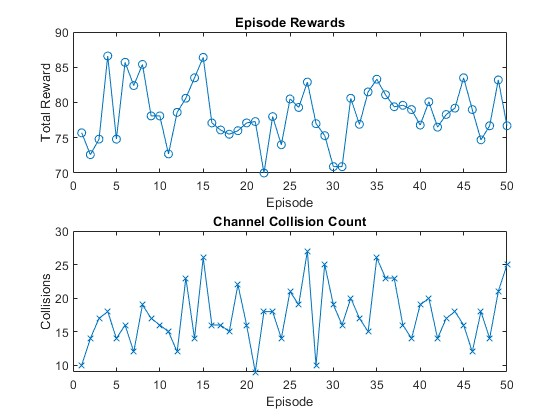
\includegraphics[width=\linewidth]{figures/collision_count_original.jpg}
        \caption{Original dataset}
    \end{subfigure}

    \caption{Performance of DQN agents trained with the four different datasets}
\end{figure}

\begin{table}[ht]
    \centering
    \caption{Comparison of Generative Models in Terms of Mean Reward and Collision Rate}
    \begin{tabular}{|l|c|c|}
    \hline
    \textbf{Model} & \textbf{Mean Reward} & \textbf{Mean Collisions per Episode} \\
    \hline
    DDPM     & 79.65   & 0.00    \\
    GAN      & 86.78   & 0.74    \\
    VQ-VAE   & 77.62   & 12.60   \\
    Original & 78.40   & 17.44   \\
    \hline
    \end{tabular}
    \label{tab:reward_collision_comparison}
\end{table}
   
    Figure 3.5 and Table 3.1 depicts the performance of DQN agents trained with datasets generated using DDPM, GAN, VQ-VAE, and the original dataset. 
    The DDPM-trained agent exhibits highly stable behavior, achieving a consistently high reward across episodes with zero collisions—indicating excellent 
    generalization and safe spectrum selection. The GAN-based agent demonstrates the highest average reward among all models; however, it incurs occasional 
    collisions, suggesting a trade-off between performance and safety. In contrast, the VQ-VAE-trained agent shows high variability in both rewards and collisions, 
    implying that its synthetic data may introduce noise or uncertainty, leading to less reliable policy learning. Lastly, the agent trained on the original dataset 
    performs moderately well in terms of reward but experiences the highest average collision rate, underscoring the benefit of augmenting training with high-quality
     synthetic data like that from DDPM. These results collectively highlight that generative models, especially DDPM, can significantly enhance the safety and 
     performance of DQN agents in dynamic spectrum access scenarios.

